\documentclass[10pt]{beamer}
\usetheme{jambro}

\title[]{Macroeconomia I - Modelo IS-LM}
\author[]{Paulo Victor da Fonseca}
\date{}

\hypersetup{
    colorlinks = true,
    urlcolor = teal,
    linkcolor = teal    
}
\usepackage[portuguese]{babel}
\usepackage{subfig}
\usepackage{emoji}
\usepackage{hyperref}

\begin{document}

\begin{frame}[plain]
    \titlepage{
        \begin{center}
            \begin{minipage}{0.8\textwidth}
                \centering
            \end{minipage}
        \end{center}}
\end{frame}

\begin{frame}{Sumário}
    \tableofcontents
\end{frame}

\section{Introdução}
\begin{frame}{Introdução}
    \begin{itemize}
        \item Aulas passadas: mercado de bens e serviços e mercados financeiros
        \bigskip
        \item Objetivo: examinar esses mercados conjuntamente e desenvolver uma estrutura para analisar como o produto agregado e a taxa de juros são determinados no curto prazo
        \bigskip
        \item Formalização do modelo IS-LM (Hicks-Hansen)
        \bigskip
        \item A versão do modelo IS-LM que estudaremos é um pouco diferente da formulação original de Hicks e Hansen.
        \bigskip
        \item Isso reflete uma mudança no modo como os bancos centrais passaram a conduzir a política monetária, transferindo o foco do controle do estoque de moeda no passado para o controle da taxa de juros no presente.
    \end{itemize}
\end{frame}

\section{Relação IS}
\subsection{Derivação da curva IS}
\begin{frame}{Derivação da curva IS}
    \begin{figure}
        \centering
        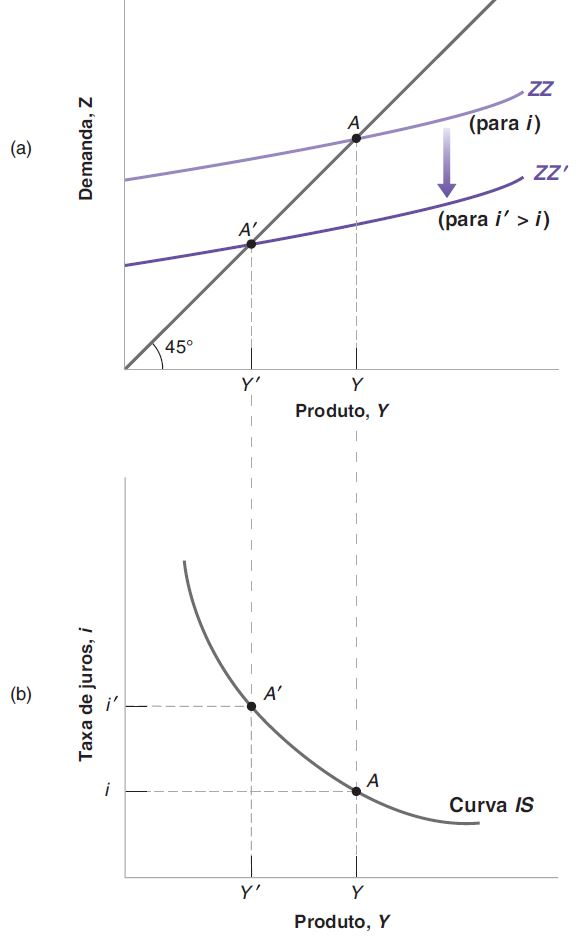
\includegraphics[width=0.27\textwidth]{./figures/aula082_fig1.JPG}
        \caption{Curva IS. Fonte: Blanchard (2017).}
        \label{IS}
    \end{figure}
\end{frame}

\begin{frame}{Derivação da curva IS}
\begin{itemize}
    \item Um aumento da taxa de juros de $i$ para $i'$ diminui o investimento
    \bigskip
    \item A diminuição do investimento leva a uma diminuição do produto, que diminui ainda mais o consumo e o investimento por meio do efeito multiplicador
    \bigskip
    \item Portanto, o equilíbrio no mercado de bens implica que um aumento da taxa de juros leva a uma diminuição do produto. Essa relação é representada pela curva IS negativamente inclinada
\end{itemize}
\end{frame}

\subsection{Deslocamentos da curva IS}
\begin{frame}{Deslocamentos da curva IS}
    \begin{itemize}
        \item Considere um aumento nos impostos de $T$ para $T'$
        \bigskip
        \item Para uma dada taxa de juros $i$, o aumento dos impostos leva a uma redução da renda disponível que, por sua vez, reduz a demanda por bens e o produto de equilíbrio
        \bigskip
        \item O nível de produto de equilíbrio diminui de $Y$ para $Y'$ e a curva IS se desloca para a esquerda
        \bigskip
        \item A dada taxa de juros, o nível de produto de equilíbrio é mais baixo do que era antes do aumento dos impostos
    \end{itemize}
\end{frame}

\begin{frame}{Deslocamentos da curva IS}
\begin{figure}
    \centering
    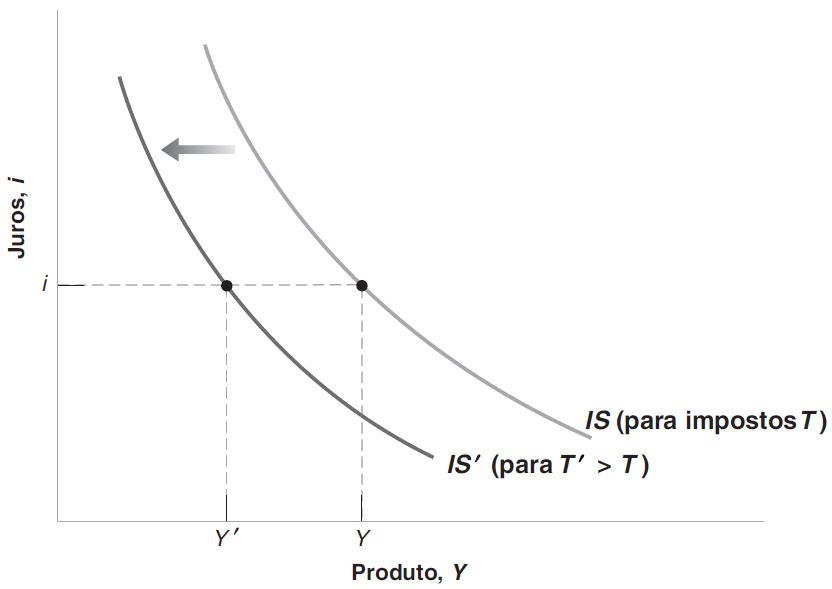
\includegraphics[width=0.6\textwidth]{./figures/aula082_fig2.JPG}
    \caption{Deslocamentos da curva IS. Fonte: Blanchard (2017).}
    \label{fig:IS2}
\end{figure}
\end{frame}

\begin{frame}{Deslocamentos da curva IS}
\begin{itemize}
    \item Generalizando, qualquer fator que, para uma dada taxa de juros, diminua o nível de equilíbrio do produto faz com que a curva IS se desloque para a esquerda
    \bigskip
    \item Simetricamente, qualquer fator que, para dada taxa de juros, aumente o nível de produto de equilíbrio desloca a curva IS para a direita
\end{itemize}
\end{frame}

\section{Relação LM}
\subsection{Moeda real, renda real e taxa de juros}
\begin{frame}{Moeda real, renda real e taxa de juros}
    \begin{itemize}
        \item Vimos que a taxa de juros é determinada pela igualdade entre oferta e demanda por moeda:
        \begin{equation}
            M = \$YL(i).
        \end{equation}
        \bigskip
        \item Será mais conveniente, aqui, reescrever a equação anterior como uma relação entre moeda real (moeda em termos de bens), renda real (renda em termos de bens) e taxa de juros:
        \begin{equation}
            \frac{M}{P} = YL(i). \tag{LM}
            \label{eq4}
        \end{equation}
        \bigskip
        \item A condição de equilíbrio nos mercados financeiros é de que a oferta real de moeda seja igual á demanda real por moeda        
    \end{itemize}
\end{frame}

\subsection{Derivação da curva LM}
\begin{frame}{Derivação da curva LM}
    \begin{itemize}
        \item Ao derivar a curva LM, temos de decidir como caracterizar a política monetária: estoque de moeda $M$ $\times$ taxa de juros $i$
        \bigskip
        \item Se instrumento de política monetária é oferta nominal de moeda $M$, então, com $P$ fixo no curto prazo, o BC fixa o estoque real de moeda $M/P$
        \bigskip
        \item Pela \ref{eq4}, um aumento na renda real leva a um aumento na demanda por moeda e a taxa de juros deve aumentar de modo que a demanda por moeda permaneça igual ao estoque de moeda
        \bigskip
        \item Dada a oferta de moeda, um aumento da renda leva, automaticamente, a um aumento na taxa de juros
    \end{itemize}
\end{frame}

\begin{frame}{Derivação da curva LM}
    \begin{itemize}
        \item Maneira mais tradicional de derivar a relação LM e a curva LM resultante
        \bigskip
        \item Embora, no passado, o instrumento de política monetária fosse a oferta de moeda, os BCs agora focam diretamente na taxa de juros
        \bigskip
        \item Eles escolhem uma taxa de juros, que chamaremos de $\bar{i}$, e ajustam a oferta de moeda para alcançá-la
    \end{itemize}
\end{frame}

\begin{frame}{Derivação da curva LM}
    \begin{figure}
        \centering
        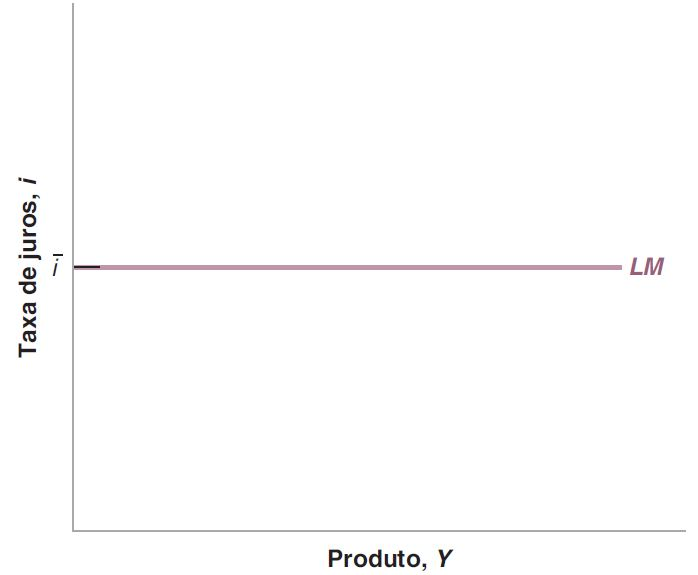
\includegraphics[width=0.5\textwidth]{./figures/aula082_fig3.JPG}
        \caption{Curva LM. Fonte: Blanchard (2017).}
        \label{fig:lm}
    \end{figure}
\end{frame}

\section{Modelo IS-LM}
\begin{frame}{Modelo IS-LM}
    \begin{itemize}
        \item A relação IS decorre do equilíbrio no mercado de bens e serviços, a relação LM do equilíbrio do mercado financeiro
        \bigskip
        \item O modelo IS-LM pode, então, ser descrito pelo sistema de equações:
        \begin{align}
            Y &= C(Y - T) + I(Y, i) + G &\qquad \text{[IS]} \nonumber \\
            i &= \bar{i} &\qquad \text{[LM]} \nonumber
        \end{align}
        \item Juntas, as curvas IS e LM determinam o produto agregado nesta economia
    \end{itemize}
\end{frame}

\begin{frame}{Modelo IS-LM}
    \begin{figure}
        \centering
        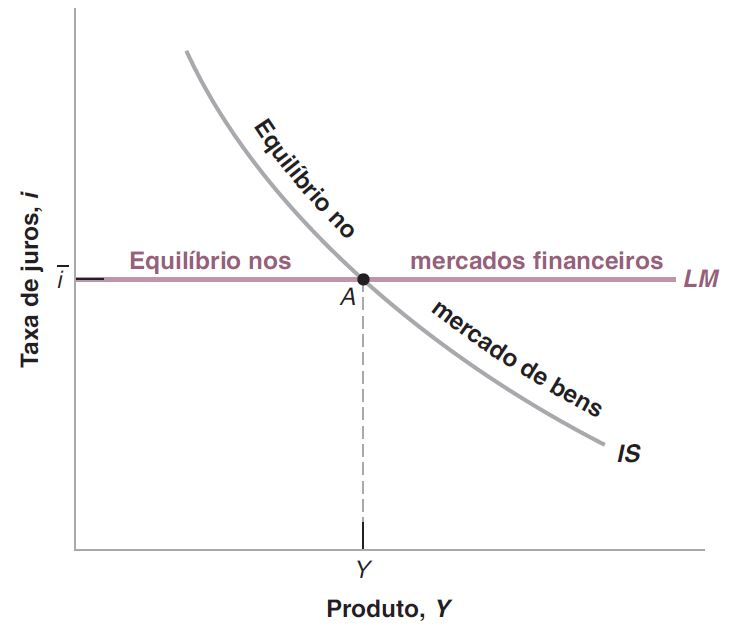
\includegraphics[width=0.5\textwidth]{./figures/aula082_fig4.JPG}
        \caption{Modelo IS-LM. Fonte: Blanchard (2017).}
        \label{fig:is-lm}
    \end{figure}
\end{frame}

\begin{frame}{Modelo IS-LM}
    \begin{itemize}
        \item Qualquer ponto sobre a curva IS corresponde a um equilíbrio no mercado de bens e serviços
        \bigskip
        \item Qualquer ponto sobre a curva LM corresponde a um equilíbrio no mercado financeiro
        \bigskip
        \item Somente no ponto $A$ ambas as condições de equilíbrio são satisfeitas simultaneamente
        \bigskip
        \item Ponto $A$ - com os níveis correspondentes de produto agregado $Y$ e taxa de juros $\bar{i}$ - temos um equilíbrio simultâneo tanto no mercado de bens quanto financeiros
    \end{itemize}
\end{frame}

\subsection{Política fiscal}
\begin{frame}{Política fiscal no modelo IS-LM}
    \begin{itemize}
        \item Suponha que o governo decida reduzir o déficit orçamentário via aumento de impostos, deixando gastos inalterados
        \bigskip
        \item Essa política de redução no déficit orçamentário é denominada \textcolor{blue}{contração fiscal} ou \textcolor{blue}{consolidação fiscal} (um aumento do déficit é chamado de \textcolor{blue}{expansão fiscal})
        \bigskip
        \item Quais os efeitos da contração fiscal sobre o produto agregado, sua composição e a taxa de juros?
        \bigskip
        \begin{enumerate}
            \item \textbf{Curva IS.} A uma dada taxa de juros, o aumento nos impostos reduz o produto agregado e, portanto, a curva IS desloca-se para a esquerda
            \bigskip
            \item \textbf{Curva LM.} Por hipótese, o BC não muda a taxa de juros desejada. Portanto, a curva LM não é deslocada e permanece em $i = \bar{i}$
        \end{enumerate}
    \end{itemize}
\end{frame}

\begin{frame}{Política fiscal no modelo IS-LM}
    \begin{figure}
        \centering
        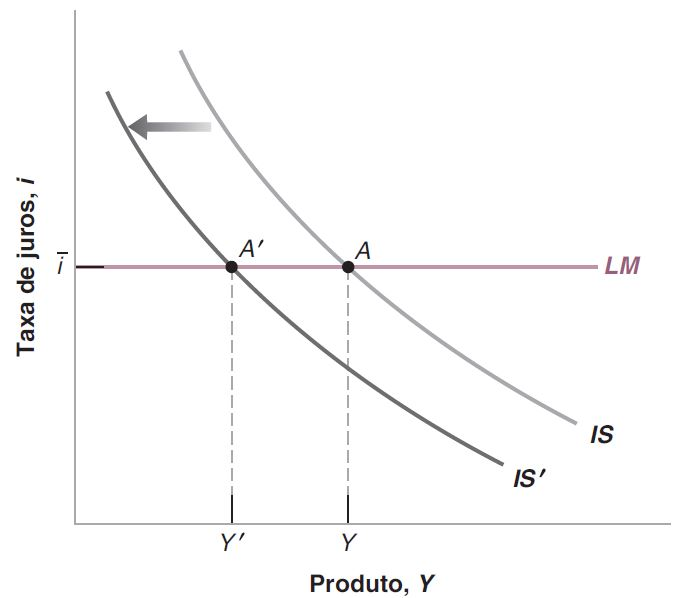
\includegraphics[width=0.5\textwidth]{./figures/aula082_fig5.JPG}
        \caption{Política fiscal contracionista no modelo IS-LM. Fonte: Blanchard (2017).}
        \label{fig7}
    \end{figure}
\end{frame}

\begin{frame}{Política fiscal no modelo IS-LM}
    \begin{itemize}
        \item Com a consolidação fiscal, a curva IS desloca-se para a esquerda, de IS para IS', e o novo equilíbrio é dado pelo ponto A'
        \bigskip
        \item O produto agregado de equilíbrio diminui de $Y$ para $Y'$
        \bigskip
        \item Como, por hipótese, a taxa de juros não se altera, à medida que a curva IS se \textbf{desloca}, a economia se move \textbf{ao longo} da curva LM, de $A$ para $A'$
    \end{itemize}
\end{frame}

\begin{frame}{Política fiscal no modelo IS-LM}
    \begin{itemize}
        \item O aumento dos impostos leva a uma redução na renda disponível o que, por sua vez, faz com que as pessoas reduzam o nível de consumo
        \bigskip
        \item Esta diminuição de demanda agregada leva, através do efeito multiplicador, a uma diminuição do produto e da renda
        \bigskip
        \item A uma dada taxa de juros, o aumento nos impostos leva, portanto, a uma diminuição do produto agregado
        \bigskip
        \item Analisando os componentes do produto: a diminuição da renda disponível e o aumento nos impostos contribuem para uma diminuição do consumo
        \bigskip
        \item A diminuição da produção leva a uma diminuição no nível de investimentos
        \bigskip
        \item Portanto, tanto consumo quanto investimento diminuem
    \end{itemize}
\end{frame}

\subsection{Política monetária}
\begin{frame}{Política monetária no modelo IS-LM}
    \begin{itemize}
        \item Vamos supor o caso de uma política monetária expansionista, na qual o BC decide baixar a taxa de juros
        \bigskip
        \item Para isto, o BC aumenta a oferta de moeda
        \bigskip
        \item Quais os efeitos de uma política monetária sobre o equilíbrio?
        \bigskip
        \begin{enumerate}
            \item \textbf{Curva IS.} A alteração na taxa de juros não muda a relação entre produção e taxa de juros. Portanto, a curva IS não é deslocada
            \bigskip
            \item \textbf{Curva LM.} Uma redução nos juros desloca para baixo a curva LM, da linha horizontal $i = \bar{i}$ para $i = \bar{i}'$
        \end{enumerate}
        \bigskip
        \item Portanto, a economia move-se para baixo ao longo da curva IS, e o equilíbrio se move do ponto $A$ para o ponto $A'$
        \bigskip
        \item O produto agregado de equilíbrio aumenta de $Y$ para $Y'$, e a taxa de juros diminui de $\bar{i}$ para $\bar{i}'$
    \end{itemize}
\end{frame}

\begin{frame}{Política monetária no modelo IS-LM}
    \begin{figure}
        \centering
        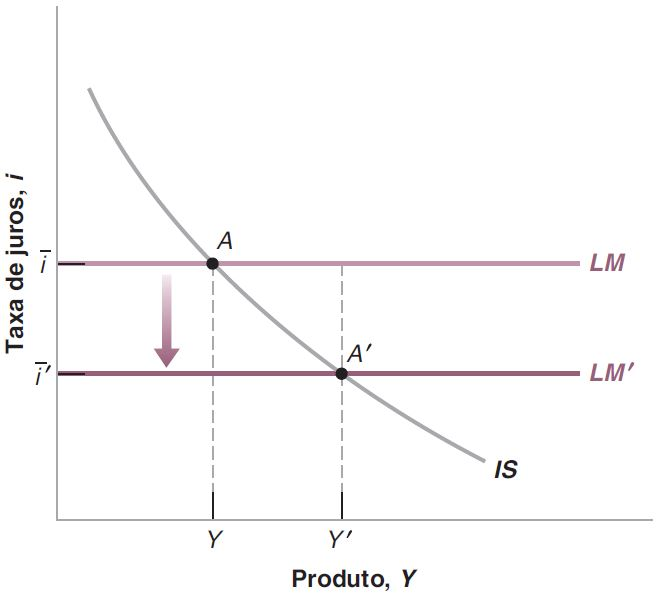
\includegraphics[width=0.5\textwidth]{./figures/aula082_fig6.JPG}
        \caption{Política monetária expansionista no modelo IS-LM. Fonte: Blanchard (2017).}
        \label{fig:polmon}
    \end{figure}
\end{frame}

\begin{frame}{Política monetária no modelo IS-LM}
\begin{itemize}
    \item Uma taxa de juros mais baixa estimula o nível de investimentos na economia o que, por sua vez, leva a um aumento na demanda agregada e do produto
    \bigskip
    \item Quanto à composição do produto agregado: o aumento do produto e a diminuição da taxa de juros levam, ambos, a um aumento dos investimentos. O aumento da renda causa um aumento da renda disponível que, por sua vez, aumenta o consumo. Portanto, tanto o consumo quanto o investimento se elevam
\end{itemize}
\end{frame}

\section{Mix de políticas}
\subsection{Mix de políticas}
\begin{frame}{Mix de políticas}
    \begin{itemize}
        \item Até agora, examinamos a condução de políticas fiscal e monetária isoladamente
        \bigskip
        \item Na prática, ambas são frequentemente usadas conjuntamente
        \bigskip
        \item O uso simultâneo de políticas monetária e fiscal é conhecido como \textcolor{blue}{combinação de políticas fiscal e monetária} ou, simplesmente, combinação de políticas (\emph{policy mix})
        \bigskip
        \item Às vezes, a combinação correta significa utilizar políticas fiscal e monetária no mesmo sentido
        \bigskip
        \item Suponha economia em recessão $\Rightarrow$ formuladores de política desejam estimular o produto
    \end{itemize}
\end{frame}

\begin{frame}{Mix de políticas}
\begin{figure}
    \centering
    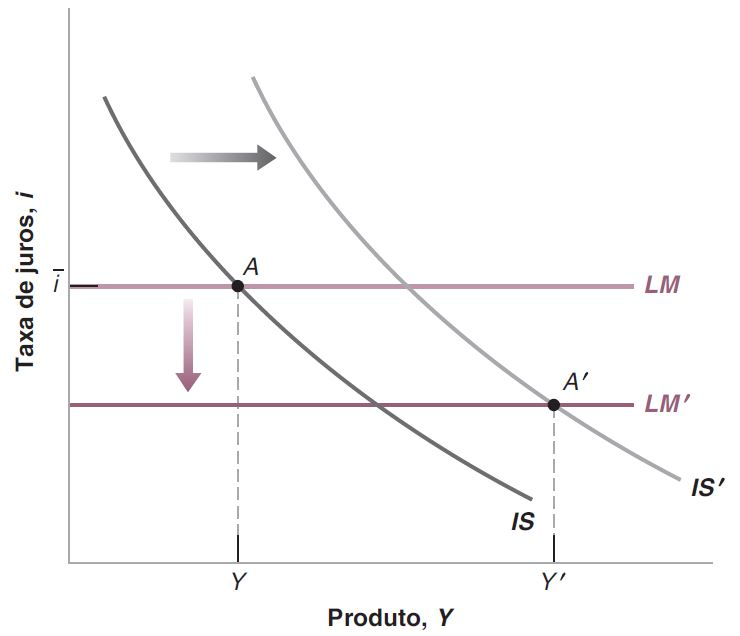
\includegraphics[width=0.5\textwidth]{./figures/aula082_fig7.JPG}
    \caption{Políticas fiscal e monetária expansionistas. Fonte: Blanchard (2017).}
    \label{fig1}
\end{figure}
\end{frame}

\begin{frame}{Mix de políticas}
\begin{itemize}
    \item Por que usar uma combinação de políticas ao invés de usar apenas um instrumento?
    \bigskip
    \begin{enumerate}
        \item[1.] Expansão fiscal $\Rightarrow$ aumento dos gastos do governo ou uma redução nos impostos (ou ambos). Elevação no déficit orçamentário. Esta elevação de déficit orçamentário aumenta a dívida pública, o que pode ser arriscado. Neste caso, é melhor confiar, ao menos em parte, na política monetária
        \bigskip        
        \item[2.] Expansão monetária $\Rightarrow$ baixar a taxa de juros. Se a taxa de juros for muito baixa, a margem para utilizar a política monetária poderá ser limitada. Neste caso, a política fiscal tem mais trabalho a fazer. Se a taxa de juros já estiver no \textcolor{blue}{limite inferior zero}, a política fiscal deverá fazer todo o trabalho
        
        %%%%%%%%%%%%%%%%%%%%%%%%%%%%%%%%%%%%%%%%
        % Inserir apêndice de armadilha da liquidez.
        %%%%%%%%%%%%%%%%%%%%%%%%%%%%%%%%%%%%%%%%
    \end{enumerate}
\end{itemize}
\end{frame}

\begin{frame}{Mix de políticas}
\begin{enumerate}    
    \item[3.] Políticas fiscal e monetária exercem efeitos distintos sobre a composição do produto. Uma redução sobre o  imposto de renda tende a aumentar o consumo em relação ao investimento. Uma redução na taxa de juros, por sua vez, afeta investimento mais que consumo. Assim, dependendo da composição inicial, formuladores de política podem querer depender mais da política fiscal ou mais da política monetária
    \bigskip
    \item[4.] Nem política fiscal nem política monetária funcionam perfeitamente. Uma diminuição dos impostos pode não aumentar o consumo. Uma diminuição nos juros pode não aumentar o investimento. Assim, é melhor usar ambas
\end{enumerate}
\end{frame}

\subsection{A recessão francesa e alemã de 2001-2002}

\begin{frame}{Recessões francesa e alemã de 2001-2002}
\begin{itemize}
    \item 2000s: nações industrializadas em quadro de declínio na atividade econômica
    \bigskip
    \item Alguns fatores podem explicar esta situação de desaceleração ou recessão:
    \medskip
    \begin{enumerate}
        \item Após o boom econômico e baixa inflação dos 1990s, era inevitável uma desaceleração e queda no emprego
        \bigskip
        \item Crise financeira asiática e crise bancária nos mercados emergentes impactaram o comércio internacional e, portanto, reduziu as exportações de nações industriais
        \bigskip
        \item O colapso da bolha especulativa da internet ou da tecnologia da informação em 2001 impactou negativamente as nações industrializadas
    \end{enumerate}
    \bigskip
    \item Como resultado destes fatores, tanto os níveis de gastos com investimento quanto consumo privado apresentaram retração, enfraquecendo o PIB entre 2001 e 2002
\end{itemize}
\end{frame}

\begin{frame}{Recessões francesa e alemã de 2001-2002}
\begin{itemize}
    \item Organização para a Cooperação e Desenvolvimento Econômico (OCDE): França e Alemanha apresentaram quadro de recessão iniciado em 2001.2 e finalizado após 9 meses
    \bigskip
    \item Sinais de lenta recuperação persistiram até 2005
    \bigskip
    \item Desaceleração que persistiu até 2005 devida, parcialmente, a fracas respostas de políticas macro
\end{itemize}
\end{frame}

\begin{frame}{Recessões francesa e alemã de 2001-2002}
    \begin{figure}
        \centering
        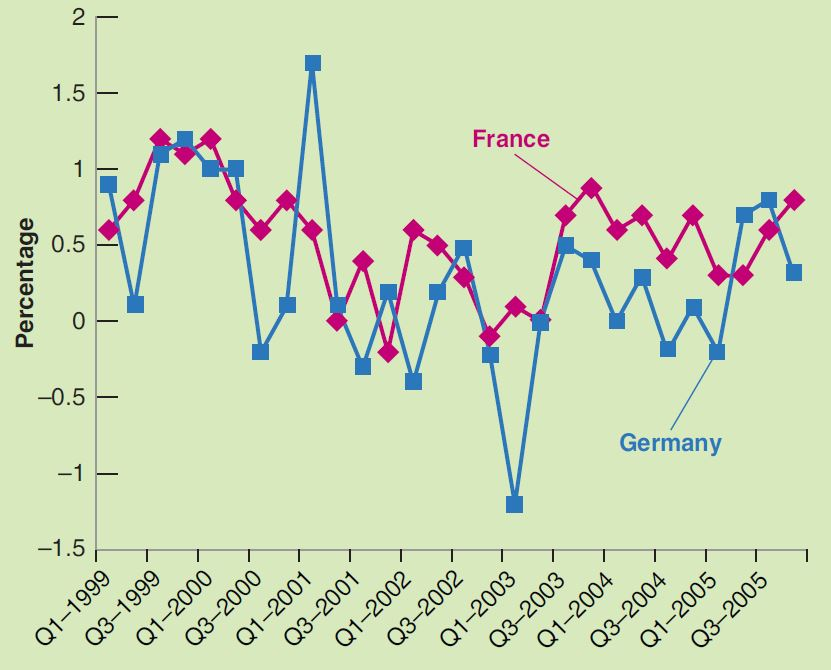
\includegraphics[width=0.55\textwidth]{./figures/aula082_fig8.JPG}
        \caption{Crescimento do PIB real (tx. trimestral) - França e Alemanha (1999-2005). Fonte: Blanchard (2017b).}
        \label{fig2}
    \end{figure}
\end{frame}

\begin{frame}{Recessões francesa e alemã de 2001-2002}
\begin{itemize}
    \item Em contraste com França, a resposta de política macro alemã foi de cortes nos gastos públicos
    \bigskip
    \item Como um estado de bem estar social, a França tem um comprometimento maior com elevados gastos públicos de bem-estar econômico
    \bigskip
    \item Alemanha, por sua vez, introduziu um conjunto de medidas impopulares de austeridade fiscal e pacotes de reformas trabalhistas - \href{https://en.wikipedia.org/wiki/Hartz_concept}{plano Hartz}
    \bigskip
    \item O chanceler alemão \href{https://en.wikipedia.org/wiki/Gerhard_Schr\%C3\%B6der}{Schröder} implementou medidas fiscais com objetivo de reduzir encargos fiscais e pressões orçamentárias do sistema de bem estar alemão em vigência
    \bigskip
    \item Reformas teriam um horizonte de 2003 a 2010, incluindo aumentos graduais nos impostos, elevações nas contribuições pensionais, cortes nos benefícios de pensões, reduções nos montantes alocados para tratamentos médicos e cortes nos benefícios de desemprego
\end{itemize}
\end{frame}

\begin{frame}{Recessões francesa e alemã de 2001-2002}
\begin{figure}
    \centering
    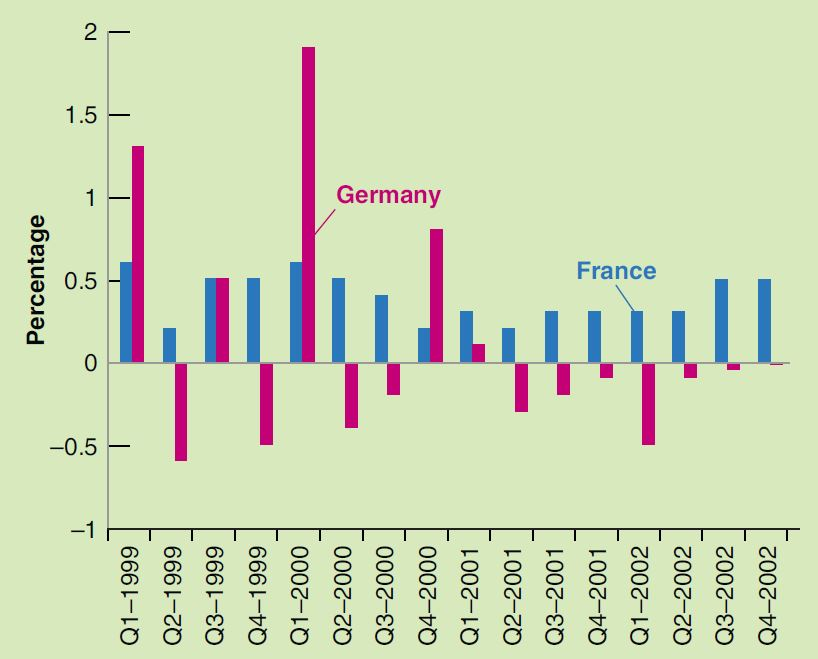
\includegraphics[width=0.5\textwidth]{./figures/aula082_fig9.JPG}
    \caption{Gastos do governo - França e Alemanha (1999-2002). Fonte: Blanchard (2017b).}
    \label{fig3}
\end{figure}
\end{frame}

\begin{frame}{Recessões francesa e alemã de 2001-2002}
\begin{itemize}
    \item Frente ao impacto potencial de uma recessão na zona do Euro, o Banco Central Europeu (ECB) adotou uma política monetária expansionista, aumentando a oferta monetária e, consequentemente, reduzindo as taxas de juros interbancárias
    \bigskip
    \item Declínio gradual nas taxas de juros: de 2\% em 1999 para 1\% em 2004
    \bigskip
    \item Essa diminuição de juros na zona do Euro foi efetiva para estimular tanto os gastos com consumo quanto com investimentos
    \bigskip
    \item Portanto, um mix de políticas fiscal e monetária foi utilizado para reduzir o impacto da recessão tanto na França quanto na Alemanha
\end{itemize}
\end{frame}

\begin{frame}{Recessões francesa e alemã de 2001-2002}
\begin{figure}
    \centering
    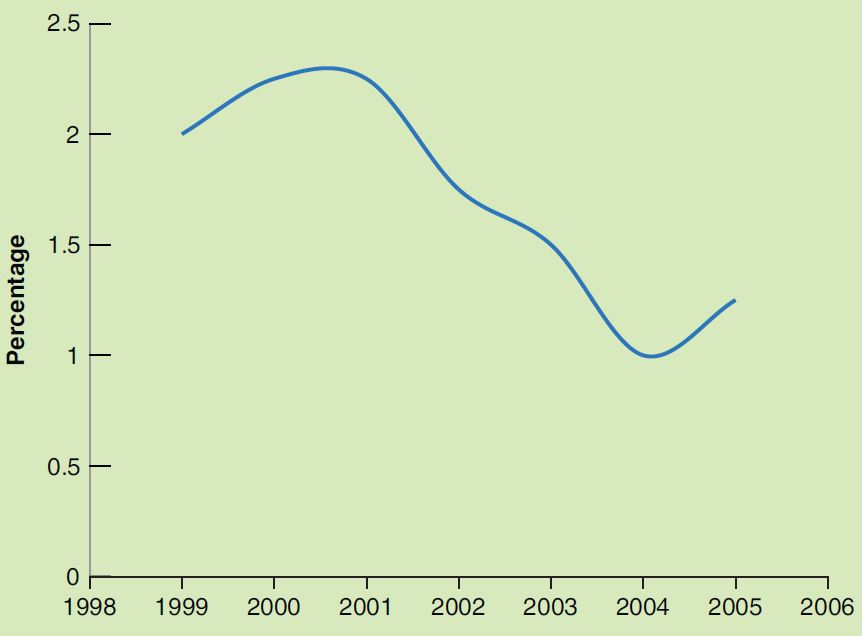
\includegraphics[width=0.55\textwidth]{./figures/aula082_fig10.JPG}
    \caption{Taxas interbancárias - ECB (1999-2005). Fonte: Blanchard (2017b).}
    \label{fig4}
\end{figure}
\end{frame}

\subsection{A recessão americana de 2001}
\begin{frame}{A recessão americana de 2001}
    \begin{itemize}
        \item Em 1992, a economia americana ingressou em uma longa expansão
        \bigskip
        \item Pelo restante da década, o crescimento do PIB foi positivo e alto
        \bigskip
        \item Em 2000, no entanto, a expansão chegou ao fim - de 2000.3 a 2001.4 o crescimento do PIB ou foi positivo e próximo a zero, ou negativo
        \bigskip
        \item Forte declínio da demanda por investimentos $\Rightarrow$ recessão. Investimento não-residencial - demanda por fábricas e equipamentos - diminuiu 4,5\% em 2001
        \bigskip
        \item Fim do período de \href{https://en.wikipedia.org/wiki/Irrational_exuberance}{``exuberância irracional''} - \href{https://en.wikipedia.org/wiki/Alan_Greenspan}{Alan Greenspan}
        \bigskip
        \item Segunda parte dos 1990s: excesso de otimisto por parte das empresas quanto ao futuro, elevando a taxa de investimento - excedendo 10\% entre 1995 e 2000
        \bigskip
        \item 2001: empresas reconheceram que otimismo era exagerado e cortaram investimentos - diminuição da demanda e, via efeito multiplicador, diminuição do PIB
    \end{itemize}
\end{frame}

\begin{frame}{A recessão americana de 2001}
\begin{figure}
    \centering
    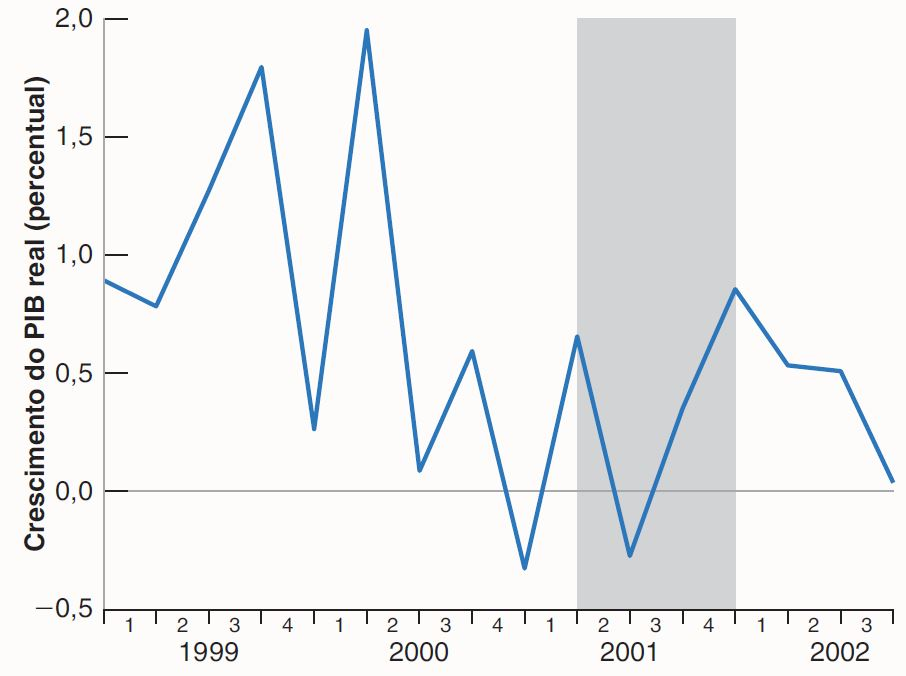
\includegraphics[width=0.5\textwidth]{./figures/aula082_fig11.JPG}
    \caption{Taxa de crescimento do PIB real - EUA (1999.1 - 2002-4). Fonte: Blanchard (2017).}
    \label{fig5}
\end{figure}
\end{frame}

\begin{frame}{A recessão americana de 2001}
\begin{itemize}
    \item Recessão poderia ter sido pior. Mas forte resposta de política macro limitou magnitude e duração
    \bigskip
    \item No início de 2001, o Fed percebeu o cenário de desaceleração e diminuiu agressivamente a taxa de juros, aumentando a oferta de moeda
    \bigskip
    \item A taxa dos fundos federais, que era de 6,5\% em janeiro, passou para menos de 2\% ao final do ano
\end{itemize}
\end{frame}

\begin{frame}{A recessão americana de 2001}
\begin{figure}
    \centering
    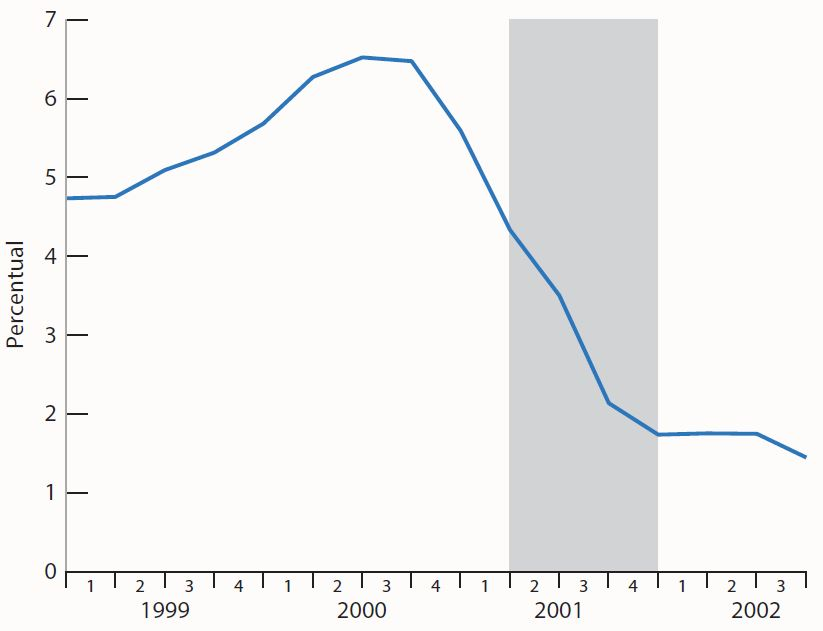
\includegraphics[width=0.5\textwidth]{./figures/aula082_fig12.JPG}
    \caption{Taxa dos fundos federais (EUA), 1999.1 - 2002.4. Fonte: Blanchard (2017).}
    \label{fig6}
\end{figure}
\end{frame}

\begin{frame}{A recessão americana de 2001}
\begin{itemize}
    \item Campanha presidencial de \href{https://en.wikipedia.org/wiki/George_W._Bush_2000_presidential_campaign}{George W. Bush} de 2000 era de impostos mais baixos
    \bigskip
    \item O argumento era o orçamento federal superavitário que possibilitaria espaço para redução de alíquota de impostos e manutenção de um orçamento equilibrado
    \bigskip
    \item A recessão de 2001 foi um motivo adicional para cortar impostos
    \bigskip
    \item Os orçamentos de 2001 e 2002 incluíram reduções substanciais nas alíquotas de impostos
    \bigskip
    \item Além disso, os ataques de 11 de setembro levaram a um aumento dos gastos, principalmente com defesa e segurança nacional
\end{itemize}
\end{frame}

\begin{frame}{A recessão americana de 2001}
\begin{figure}
    \centering
    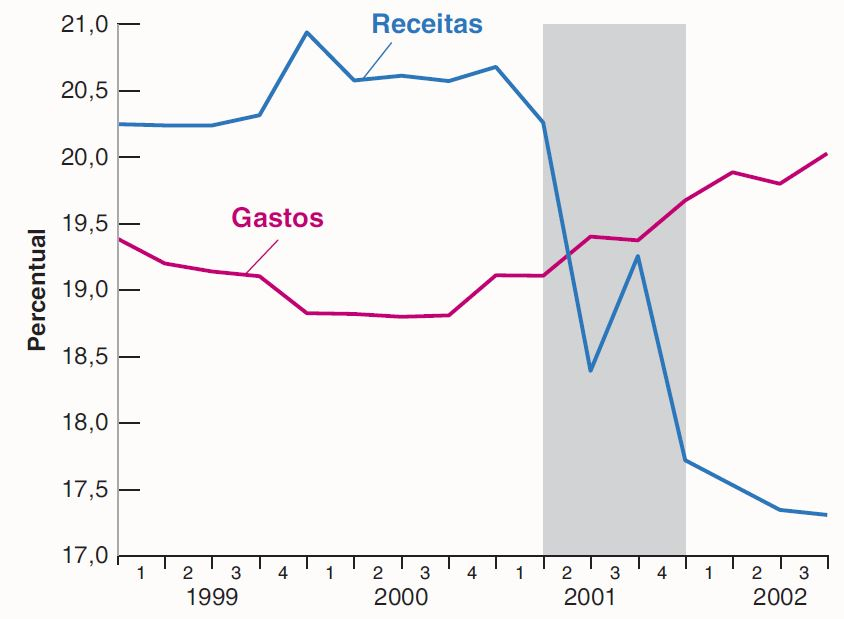
\includegraphics[width=0.55\textwidth]{./figures/aula082_fig13.JPG}
    \caption{Receitas e gastos do governo federal dos EUA (\% PIB), 1999.1 - 2002.4. Fonte: Blanchard (2017).}
    \label{fig7}
\end{figure}
\end{frame}

\subsection{Mix de políticas}
\begin{frame}{Mix de políticas}
    \begin{itemize}
        \item Às vezes, a combinação certa de políticas é usar políticas fiscal e monetária em direções opostas, e.g., combinação de consolidação fiscal com expansão monetária
        \bigskip
        \item Suponha que o governo tenha um grande déficit orçamentário e que pretenda reduzi-lo, mas sem desencadear uma recessão
    \end{itemize}
\end{frame}

\begin{frame}{Mix de políticas}
\begin{figure}
    \centering
    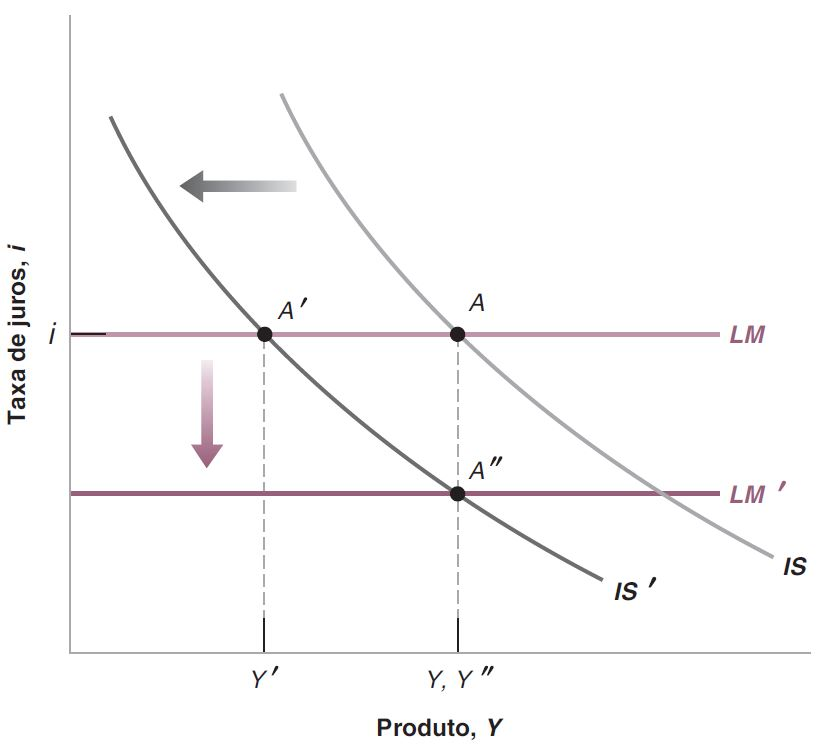
\includegraphics[width=0.5\textwidth]{./figures/aula082_fig14.JPG}
    \caption{Combinação de consolidação fiscal e expansão monetária. Fonte: Blanchard (2017).}
    \label{fig8}
\end{figure}
\end{frame}

\begin{frame}{Mix de políticas}
\begin{itemize}
    \item O que acontece com a composição do PIB neste caso?
    \bigskip
    \item No caso do consumo, isto depende da forma como o déficit é reduzido
    \bigskip
    \item Se a redução tomar forma de uma diminuição de gastos públicos, a renda permanece inalterada, a renda disponível permanece inalterada e, assim, o consumo permanece inalterado
    \bigskip
    \item Se a redução tomar a forma de um aumento de impostos, a renda disponível é mais baixa, bem como o consumo
    \bigskip
    \item O que acontece com o investimento não é ambíguo: um produto inalterado e uma taxa de juros mais baixa implica em um nível de investimentos mais alto
\end{itemize}
\end{frame}

\begin{frame}{Mix de políticas}
\begin{itemize}
    \item Combinação de políticas usada por Bill Clinton no início dos 1990s
    \bigskip
    \item Uma das prioridades era reduzir o déficit orçamentário com uma combinação de corte de gastos e aumentos de impostos
    \bigskip
    \item Preocupação de que contração fiscal levaria a uma diminuição da demanda e desencadearia outra recessão
    \bigskip
    \item A estratégia certa era combinar uma contração fiscal com uma expansão monetária
    \bigskip
    \item Esta foi a estratégia adotada por Bill Clinton (política fiscal) e Alan Greenspan (política monetária)
    \bigskip
    \item O resultado, combinado com um pouco de sorte econômica, foi uma redução constante do déficit orçamentário (que ficou superavitário no final da década de 1990) e um aumento constante do produto durante o restante da década
\end{itemize}
\end{frame}

\section{Como o IS-LM se ajusta aos fatos?}
\subsection{Como o modelo IS-LM se ajusta aos fatos?}
\begin{frame}{Como o modelo IS-LM se ajusta aos fatos?}
    \begin{itemize}
        \item Até agora ignoramos a dinâmica de ajustamento da economia
        \bigskip
        \item O ajuste do produto leva algum tempo. Para captar essa dimensão temporal, precisamos reintroduzir a dinâmica
        \bigskip
        \item É provável que os consumidores levem algum tempo para ajustar seu consumo após mudanças na renda disponível
        \bigskip
        \item É provável que empresas levem tempo para ajustar gastos com investimento após mudanças nos níveis de vendas e/ou taxas de juros
        \bigskip
        \item É provável que empresas levem tempo para ajustar os níveis de produção após mudanças em suas vendas
    \end{itemize}
\end{frame}

\begin{frame}{Como o modelo IS-LM se ajusta aos fatos?}
\begin{itemize}
    \item Em resposta a aumento de impostos, leva algum tempo para que os gastos de consumo respondam à diminuição da renda disponível, mais algum tempo para que a produção diminua em resposta à diminuição dos gastos em consumo, mais tempo ainda para que o investimento diminua em resposta a vendas mais baixas, para que o consumo diminua em resposta à mudança induzida na renda, e assim por diante
    \bigskip
    \item Em resposta a uma redução na taxa de juros, leva algum tempo para que os gastos de investimento respondam à diminuição nos juros, mais algum tempo para que a produção aumente em resposta a um aumento da demanda, e mais tempo ainda para que o consumo e o investimento aumentem em resposta à mudança no produto, e assim sucessivamente
\end{itemize}
\end{frame}

\begin{frame}{Como o modelo IS-LM se ajusta aos fatos?}
\begin{itemize}
    \item Efeitos de uma decisão do Fed de aumentar a taxa dos fundos federais em 1\%
    \bigskip
    \item Exercícios econométricos conduzidos com dados da economia EUA para o período de 1960 a 1990
    \bigskip
    \item Um aumento nas taxas de fundos federais reduzem as vendas no varejo ao longo do tempo. A maior diminuição das vendas no varejo, -0,9\%, ocorre após 5 trimestres
    \bigskip
    \item Vendas mais baixas levam a um produto mais baixo. Em resposta à diminuição das vendas, as empresas cortam sua produção, mas menos do que a diminuição das vendas - empresas acumulam estoques por algum tempo. O ajuste da produção é mais suave e lento do que o das vendas. A maior queda (-0,7\%) é alcançada ao fim de 8 trimestres. São necessários cerca de 2 anos para que a política monetária tenha seu efeito total sobre o produto
\end{itemize}
\end{frame}

\begin{frame}{Como o modelo IS-LM se ajusta aos fatos?}
\begin{figure}
    \centering
    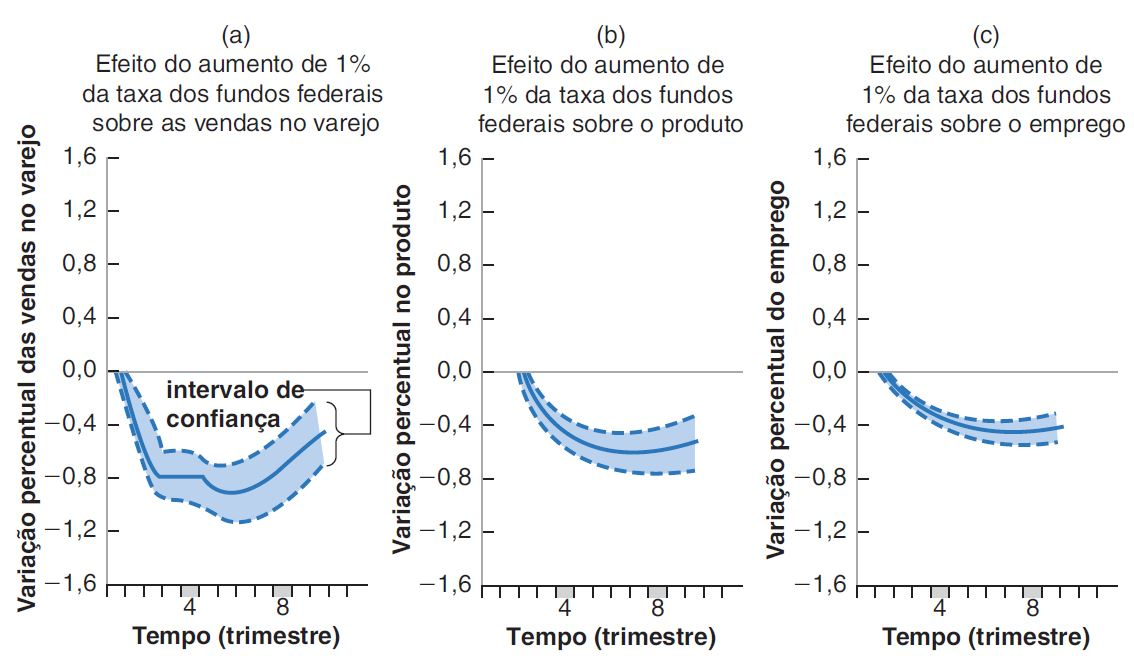
\includegraphics[width=0.7\textwidth]{./figures/aula082_fig15.JPG}
    \caption{Efeitos empíricos de um aumento na taxa dos fundos federais. Fonte: Blanchard (2017).}
    \label{fig9}
\end{figure}
\end{frame}

\begin{frame}{Como o modelo IS-LM se ajusta aos fatos?}
\begin{itemize}
    \item Um produto mais baixo leva a um emprego mais baixo. Quando as empresas cortam a produção, também cortam o emprego. A diminuição do emprego é lenta e contínua, alcançando -0,5\% depois de 8 trimestres
    \bigskip
    \item Uma das hipóteses do modelo IS-LM é de que o nível de preços é fixo no curto prazo, portanto, não se altera em resposta a mudanças na demanda
    \bigskip
    \item A figura mostra que esta hipótese não é uma aproximação ruim da realidade no curto prazo. O nível de preços praticamente não se altera nos  primeiros seis trimestres. Somente após esse período que o nível de preços parece diminuir
\end{itemize}
\end{frame}

\begin{frame}{Como o modelo IS-LM se ajusta aos fatos?}
\begin{figure}
    \centering
    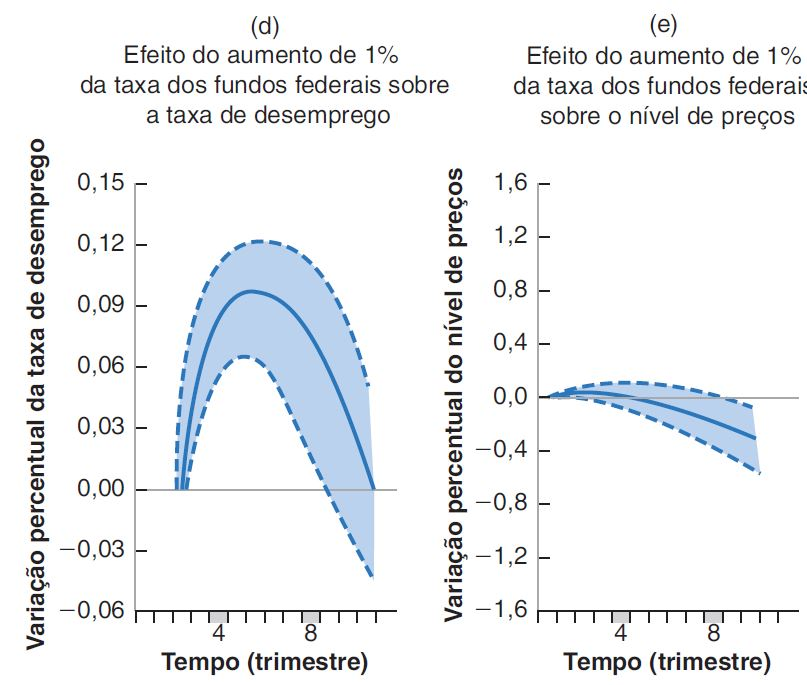
\includegraphics[width=0.5\textwidth]{./figures/aula082_fig16.JPG}
    \caption{Efeitos empíricos de um aumento na taxa dos fundos federais. Fonte: Blanchard (2017).}
    \label{fig10}
\end{figure}
\end{frame}

\section{Bibliografia}
\begin{frame}{\emoji{books} Bibliografia}
    \begin{itemize}
        \item BLANCHARD, O. Macroeconomia. 7.ed. São Paulo: Pearson Education do Brasil, 2017a\medskip        
        \item BLANCHARD, O. Macroeconomics. 7.ed (Global edition). Essex: Pearson Education Limited, England 2017b
    \end{itemize}
\end{frame}
\end{document}